\section{Aufbau}
\label{sec:Aufbau}

\begin{figure}[H]
         \centering
         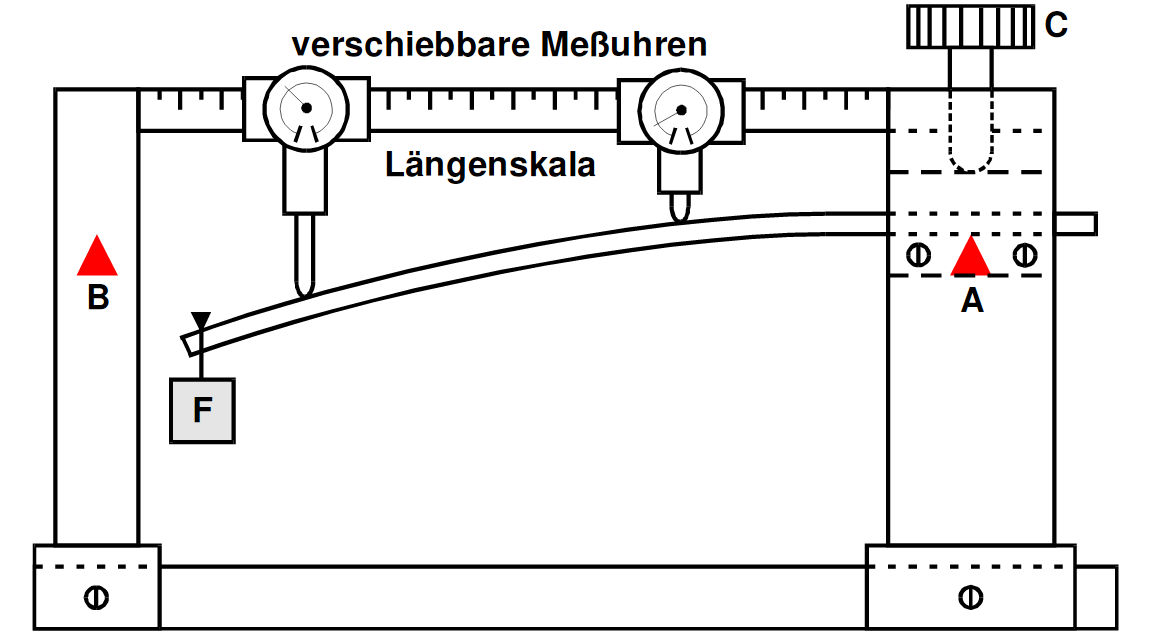
\includegraphics[width=\linewidth-150pt,height=\textheight-150pt,keepaspectratio]{content/Bilder/aufbau.png}
         \caption{Messapperatur zur Bestimmung des Elastizitätsmoduls $E$ aus einer Biegung des Materials. \cite{V103}.}
         \label{fig:Aufbau}
       \end{figure}

Die Messapparatur besteht aus einer Einklemmvorrichtung, an welcher die Stabenden horizontal befestigt werden können.
Um den Stab einer konstanten Normalspannung zu unterwerfen wird ein Gewicht verwendet,
 welches am offenen Stabende bzw. der Stabmitte befestigt wird. Oberhalb des Stabes ist eine
 Längenskala befestigt. Auf dieser liegen zwei Messuhren mit einer Genauigkeit von  $\SI{10}{\micro\meter}$, welche
 über die gesamte Stablänge verschoben werden können.
